%# -*- coding: utf-8-unix -*-
%%==================================================
%% chapter01.tex for SJTU Master Thesis
%%==================================================

%\bibliographystyle{sjtu2}%[此处用于每章都生产参考文献]
\chapter{绪论}
\label{chap:intro}

\section{水军问题相关现状}

近年来随着信息网络和智能便携设备高速发展,人们的网络生活变化日新月异。与此同时,人们的衣食住行也和网络不断产生着联系。一方面,由于网络消费方便快捷,社交网络信息传播速度快的特点,越来越多的人选择通过网络进行社交和消费行为。中国互联网络信息中心发布的第41次《中国互联网络发展状况统计报告》显示:截止2017年12月,中国网民规模达7.72亿,其中手机上网人数占比达97.5\%;移动支付规模持续扩大,网民在线下消费使用手机网上支付比例由2016年底的50.3\%提升至65.5\%;电子商务持续快速增长,2017年1月至11月电子商务平台收入2188亿元,同比增长高达43.4\%。在世界范围内,2018年We Are Social和Hootsuite的最新全球数字报告显示,世界网民规模达到了40亿,其中使用智能手机上网的人数占比达52\%;Statista最新数据显示,2017年的电商市场年度总支出达到了近1.5万亿美元。全球范围内,使用电商平台购买商品(如衣服、食品、电子产品和玩具)的人数增长了8%,全球近18亿人在网上购物,占所有互联网用户的45%左右。另一方面,各种网络平台也在飞速发展。在中国范围内,淘宝\footnote{www.taobao.com}是深受欢迎的网购零售平台,拥有近5亿的注册用户数,每天有超过6000万的固定访客,同时每天的在线商品数已经超过了8亿件,平均每分钟售出4.8万件商品;大众点评\footnote{www.dianping.com}是一家独立第三方消费点评网站。大众点评不仅为用户提供商户信息、消费点评及消费优惠等信息服务,同时亦提供团购、餐厅预订、外卖及电子会员卡等线上到线下交易服务;微博\footnote{www.weibo.com}是中国广受欢迎的社交网络平台,是一个基于用户关系信息分享、传播以及获取的平台。用户可以用140字的文字更新信息,并实现即时分享。而在世界范围内,亚马逊\footnote{www.amazon.com}是网络上最早开始经营电子商务的公司之一,现在已成为全球商品品种最多的网上零售商和全球第二大互联网企业;Yelp\footnote{www.yelp.com}是发源于美国,现世界最著名的商户点评网站,囊括各地餐馆、购物中心、酒店、旅游等领域的商户;而Facebook\footnote{www.facebook.com}稳座世界范围社交网络头把交椅,拥有近20亿活跃使用者。可以说,网络消费平台和社交网络平台对人们的日常生活有着十分重要的作用。

\begin{figure}[htp]
	\centering
	\subcaptionbox{“紫光阁地沟油”事件\label{figure:spam-a}} %标题的长度,超过则会换行,如下一个小图。
	{
\includegraphics[height=9cm]{intro-2.jpg}}
	\hspace{4em}
	\subcaptionbox{微博水军刷转发量\label{figure:spam-b}}
	{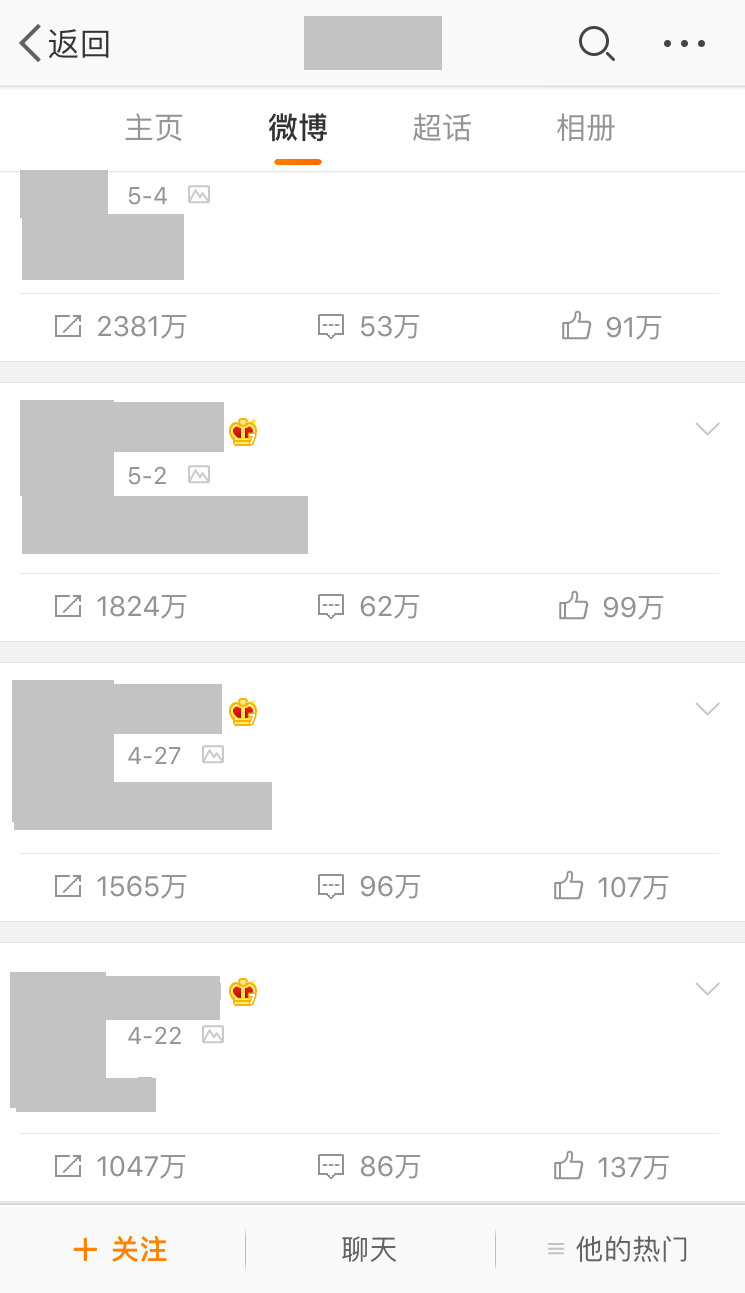
\includegraphics[height=9cm]{intro-3.png}}
	\caption[网络水军的表现]{网络水军的表现}
\end{figure}

但是,在利益的驱使下,如此庞大的市场中必然会出现秩序的破坏者。这些破坏者就是水军。他们依靠控制的大量账号,在社交网络中为雇主造势,在网购平台中恶意刷单,在评论网站中发布虚假的点评内容,以满足雇主的需求并获得利益。普通的网民在从众心理的诱导下,很容易被水军发布的言论所误导,对社交网络中的热点话题产生误解,或者在网络消费过程中蒙受经济损失。网络水军们甚至形成了成熟的黑色产业链:微博买粉丝买热搜,淘宝恶意刷单,大众点评刷好评,微信公众号刷流量等。低价雇佣真实用户进行水军行为的广告网络上也随处可见。水军的存在对当前的网络环境造成了恶劣的影响,是伴随着时代进步产生的新问题。水军们可以颠倒黑白将国家党建宣传机关说成卖地沟油的黑心饭店(如图~\ref{figure:spam-a}),也可以帮雇主疯狂地刷转发量(如图~\ref{figure:spam-b})。可以预见近期内,水军的检测在世界范围内都将是一项挑战。


尽管水军检测相关的研究已经进行了很多年,并且在NLP(Natural Language Processing)领域是一个老生常谈的问题,但是从安全和隐私角度来考虑的话,水军检测问题还有很多未经发掘的地方。伴随着机器学习和人工智能近年来的高速发展,机器学习+安全的新思维可以带给我们更多解决问题的思路。表~\ref{tbl:intro-1}列举了截至2018年5月在Elsevier电子期刊全文(ScienceDirect)数据库和中国知网(CNKI)数据库内检索2012年以来世界上和中国国内的以“水军检测/安全”为题目或关键词的论文数。从表中数据可知,国际上对水军检测的安全问题关注程度逐渐增加,但相关的发表很少,而国内更是进展缓慢。本次毕业设计选题时也考虑到了希望在该领域能够有所开拓,能够吸引更多的人来研究这个严重的当代社会问题。

\begin{table}[htb]
	\centering
	\caption[以“水军检测/安全”为题目或关键词的论文数目]{以“水军检测/安全”为题目或关键词的论文数目}
	\label{tbl:intro-1}
	\begin{tabular}{c|ccccccc}	
		\toprule
						& 2012 & 2013 & 2014 & 2015 & 2016 & 2017 & 2018 \\
		\midrule
		CNKI 			& 0   & 1   & 4   &	12  & 5   & 10  &   1 \\
		ScienceDirect	& 100 & 201 & 154 &	167 & 172 & 194 & 111 \\
		\bottomrule
	\end{tabular}
\end{table}

\section{O2O网络平台中的人工水军问题}

在众多网络平台中,O2O(Online To Offline)平台是一个重要组成部分。O2O是指线上到线下,即使用线上的宣传来刺激顾客进行线下活动的消费,然后利用线下活动的反馈促进该活动线上的宣传效果 \cite{Wei:2014}。上文提到的大众点评和Yelp都属于O2O平台。作为O2O平台重要的反馈部分,消费者的评论可以给打算消费的人提供重要的参考价值,帮助他们做出消费决定。这些评论表达出的观点对于目标店铺的声誉和营业额至关重要。优质的、详细的、正面的评价可以为商家带来名声和利益,而负面的评价会让后来者望而却步。于是在利益的驱动下,虚假评论和水军们出现了。商家们为了吸引更多的潜在顾客,雇佣一批账号对自己的店铺进行正面的评价以提升声誉,以及编写虚假的消费体验以欺骗那些打算在这些店铺进行消费的顾客们。此外,更有无良的商家会雇佣水军去恶意差评自己的竞争对手们\cite{Gupta:2017}。这种雇佣水军的行为已经成为了网店商家见公开的秘密。而且,快速发展的社交平台使得水军的存在形式也飞速进化,对社会产生的恶劣影响也越来越严重\cite{CHAKRABORTY:2016}。饱受水军困扰的大众点评就建立了自己的专职处理作弊和炒作、虚假点评的过滤系统,并多次联合警方打击第三方炒作机构。Yelp也起诉过两家“名誉管理公司”,指控他们刷好评引起商家间的不公平竞争。但是,尽管平台逐渐加大水军的打击力度,水军仍然不停地出现,甚至有越发猖獗的趋势。水军产业链已然成熟,他们对于如何躲避平台检测系统已经轻车熟路。寻找新的水军检测方法是一项十分迫切的需求。

如果将水军检测问题抽象化,该问题可以简化为二分类问题。给定一系列账户及其相关信息,如何寻找一个新颖高效的分类方法。每一个账户都拥有丰富的信息:评论信息可以反映一个用户撰写过的所有评论、对商家的打分等;时间信息可以反映一个用户何时注册的账号、在何时发表过评论等;位置信息可以反映一个用户评论过的商家位置、在哪里签过到等;个性化信息,例如个人资料完成度、自定义头像、个性签名等,可以反映一个用户对该账户的自定义程度。而处理这些信息的方法也多种多样:NLP擅长处理文本信息,可以分析文本的相似程度;机器学习算法可以根据样本的特征做出分类预测,但是需要足够多的训练样本;新兴的深度学习表现优异,但是如何构建训练网络十分关键。由于文本分析的方法已经过时,故不再进一步讨论。于是问题的关键部分即是账户特征的选取和分类方法的选择。能够充分反映水军账户和正常账户区别的的特征配合上高效的分类方法,对于问题的解决十分关键。此外还需要注意的是,在现实中水军用户数量和正常用户数量差距悬殊,在检测水军的过程中不可避免地会产生错误预测,从而导致对正常用户的“误伤”或放过了真的水军。如何减少出错率也非常关键。若一个模型可以检测出绝大部分的水军,但同时会将大量正常用户也判定为水军,那么这个模型是不可用的。同理,如果一个模型误判率很低,但检测水军的效率也很低,那这个模型同样也是不可用的。如何达到二者之间的平衡,也是我们需要关注的地方。

本次毕业设计将主要关注账户特征的选取和分类方法的选择,并在此基础上设计一个准确率和误判率平衡的检测模型。

\section{前人对水军检测的研究}

\begin{figure}[h]
	\centering
	\subcaptionbox{早期机器水军示例\label{figure:bot-a}} %标题的长度,超过则会换行,如下一个小图。
	{
\includegraphics[height=8cm]{intro-1.jpg}}
	\hspace{4em}
	\subcaptionbox{受雇人工水军示例\label{figure:bot-b}}
	{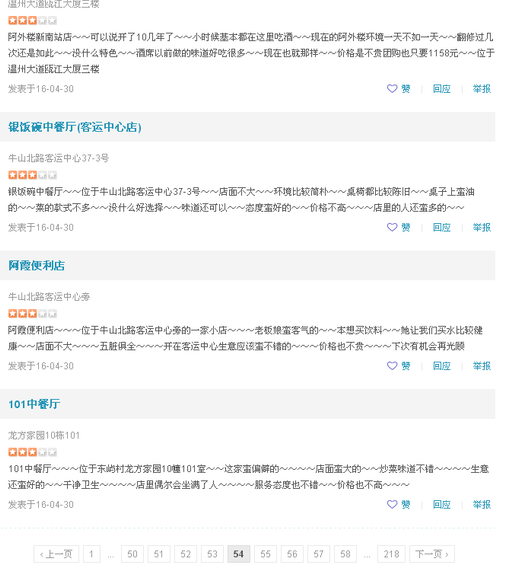
\includegraphics[height=8cm]{intro-4.jpg}}
	\caption[水军示例]{水军示例}
\end{figure}

水军检测方面的研究已经进行了数年\cite{Spirin:2012}。早期的水军形式非常基础,基本是脚本批量控制的机器水军,内容也非常简单,很容易人工辨别。如图~\ref{figure:bot-a}是典型的早期机器水军形式,其特点是用户名无意义或使用默认用户名,没有个性化信息(自定义头像等),使用大量不同的账号在短时间内发表几乎相同的内容等。这类早期机器水军由于特点鲜明,欺骗性低,很容易通过分析评论内容的方法分辨出来。早期的研究者们提出了许多基于文本的词法分析和语法分析方法,也有一些通过将评论和评论者特征应用于简单的机器学习算法来查找可疑账户的方法。Mukherjee等人 \parencite{Mukherjee:2013}分别利用词法分析方法和表现特征方法进行Yelp里的水军检测。在研究者们进行科研的同时,网络商业平台们也意识到了水军的危害性,并建立了各自的检测系统以过滤低质量评论和疑似水军评论。这些系统帮助维护了评论环境,但也促使水军技术的不断进步。机器水军逐渐落伍,人工水军凭借其隐蔽性优势逐渐成为水军主流。能够欺骗平台检测系统的水军技术层出不穷,甚至Yao等人 \parencite{Y.Yao:2017}研究出了用RNN(Recurrent Neural Networks)自动生成水军评论的方法,而且可以通过学习正常用户评论内容和控制生成速率的方法,躲避平台过滤系统的侦查。如图~\ref{figure:bot-b}就是大众点评上受雇佣的人工水军示例。单独来看每一条评论似乎与正常用户区别不大,但如果查看该用户每一条点评的时间就会发现他在一天只内写了数十条点评内容,这显然是不符合常理的。 在日益更新的水军技术面前,之前过时的水军检测技术急需更新。水军检测领域的着眼点也逐渐从文本分析转移到了模式提取和特征分析,时间、排名、话题度和活跃程度等特征也证明了它们检测水军的能力。这些新思路为水军检测领域提供了新的方向。Santosh等人 \parencite{Santosh:2016}在Yelp上分析了水军活动爆发出现的时间顺序和发生速率,并在此基础上提出了一个向量自回归(Vector AutoRegression)模型来预测水军活动的发生。他们认为水军的活动具有短时间内爆发的特征。这有这有才可以迅速达成水军们宣传雇主的目标。故这个爆发点可以用来预测水军的活动。Nilizadeh等人 \parencite{Nilizadeh:2017} 设计了一个利用用户喜好的话题来判别推特\footnote{www.twitter.com}中的可疑水军用户的模型。他们假设一个特定群体的用户所偏好的话题是固定的。若一个用户突然发布了一个他不偏好的话题的内容,那么他的身份就很可疑。

\section{SpamTracer水军检测模型}

本次毕业设计在前人工作的基础上,提出了自己的水军检测模型——\emph{SpamTracer}。该模型最大的特点是利用了地理位置特征。地理位置特征在水军检测方面具有很大的潜力。在O2O平台中,每家店铺都具有位置信息。用户评论过的所有店铺按照时间顺序形成序列,这些店铺的位置也会形成序列。无论是水军用户还是正常用户,只要参与过评论,都会形成这样的位置序列。但是,水军用户在进行水军活动的时候不会注意目标店铺的位置顺序,相邻店铺间的位置关系会比正常情况下更加复杂,即出现“绕远路”的现象。而普通用户评论种店铺的位置顺序是符合人类生活规律的。二者截然不同的行动理念产生的结果就是在地理位置相关特征的统计数据和分布情况上出现很大的差异。这种差异可以成为我们检测水军用户的切入点。而且,位置相关的特征难以伪造,可以有效防止水军绕开检测系统。通过在一个有标签的用户评论数据集上进行计算,我们发现水军用户和普通用户在地理特征上都表现出了双峰分布的特点。我们调整了SpamTracer模型使它能够完美契合这样的分布特点。

一些已经发表的工作也讨论过地理位置特征在水军检测方面的可能性。Zhang \parencite{Zhang:2014}等人在社交网络OSN(Online Social Networks)中利用地理位置特征检测水军账号。他们结合了账户特征(姓名、性别、评论数等)和位置信息,利用信息熵(Information Entropy)将二者结合进行判断。Gong等人 \parencite{Gong:2018}在基于位置的社交网络LBSN(Location-Based Social Networks)中收集了用户的签到(check-in)信息,然后利用LSTM(Long Short-Term Memory)神经网络分析这些签到信息,并在模型测试中展示出了极高的准确率。这些工作启发了我们,位置信息具有极大的潜力。我们的SpamTracer将使用全新的方法处理位置信息,并让这些特征在水军检测过程中起到关键作用。

除了水军检测以外,本次毕业设计还讨论了关于水军检测模型的应用。由于模型需要有大量的数据作为基础才能进行判断,而对于一般用户来说,并没有使用模型的条件。故我们可以利用SpamTracer分析水军用户们发动水军活动的时间规律和地点规律,这样就可以在一定程度上帮助普通用户鉴别水军。经过研究,我们发现网络商铺雇佣水军的行为确实存在一些时间规律和地点规律。例如:网络商铺倾向于在刚刚开业的时候雇佣水军帮助他们的店铺积累人气,并在平台的搜索系统中获得较高的排名。这样这些商铺就更有可能吸引到浏览的人的注意力,并获得更多的营业额。


\section{本次毕业设计的主要贡献}

本次毕业设计的主要贡献如下列出:

\begin{enumerate}
	\item[(1)] 我们使用地理位置特征在O2O商业平台中进行水军评论检测。我们收集了店铺的地理位置信息,按照时间顺序将属于同一个人点评过的店铺的位置信息整理在一起,形成地理位置特征序列。
	\item[(2)]  我们建立了一个特别的SpamTracer模型,用于描述水军用户和普通用户在地理位置特征上的分布差异。SpamTracer分析地理位置特征序列,然后对该用户所属身份(水军用户或普通用户)做出判断。
	\item[(3)]  我们提出了三个重要的水军行动的关于时间地点的命题。我们的实验结果证实了这些命题并给出了合理的解释。
\end{enumerate}

本文剩下的部分将按照如下说明开展:第二章介绍相关基础知识,包含机器学习相关、网络诈骗中的分类算法和隐马尔可夫模型简介;第三章介绍地理位置特征的具体提取步骤,并论述该特征的合理性;第四章介绍SpamTracer模型的建立过程,并论述该模型理论上的可行性;第五章介绍SpamTracer模型的应用,提出三条水军行动规律,并设计实验验证这些规律;第六章介绍模型的测试过程,包括数据集情况简介、实验环境描述、水军检测功能的测试结果及分析,以及水军行动规律分析实验的结果。最后,第七章得出结论,总结整个毕业设计。




